\documentclass{article}
\usepackage[utf8]{inputenc} %codificacion de caracteres que permite tildes
% \usepackage[spanish]{babel}

% \usepackage{amsfonts}
% \usepackage{natbib}
% \usepackage{amsmath}
% \usepackage{amssymb}
% \usepackage{mathrsfs} % Cursive font
% \usepackage{ragged2e}
\usepackage{fancyhdr}
% \usepackage{nameref}
% \usepackage{wrapfig}
\usepackage{hyperref}


\usepackage{float}
\usepackage{graphicx}
\usepackage{subcaption}
% \graphicspath{ {./Resources/} }

% \usepackage[
% top    = 2cm,
% bottom = 1.5cm,
% left   = 1.5cm,
% right  = 1.5cm]
% {geometry}




\usepackage{mathtools}
\usepackage{xparse} \DeclarePairedDelimiterX{\Iintv}[1]{\llbracket}{\rrbracket}{\iintvargs{#1}}
\NewDocumentCommand{\iintvargs}{>{\SplitArgument{1}{,}}m}
{\iintvargsaux#1}
\NewDocumentCommand{\iintvargsaux}{mm} {#1\mkern1.5mu,\mkern1.5mu#2}

\makeatletter
\newcommand*{\currentname}{\@currentlabelname}
\makeatother



\addtolength{\textwidth}{0.2cm}
\setlength{\parskip}{8pt}
\setlength{\parindent}{0.5cm}
\linespread{1.5}

\pagestyle{fancy}
\fancyhf{}
\rhead{TP Lógica Borrosa - Cipullo, Sullivan}
\lhead{Introducción a la Inteligencia Artificial}
\rfoot{\vspace{1cm} \thepage}

\renewcommand*\contentsname{\LARGE Índice}

\setlength{\skip\footins}{0.5cm}


\begin{document}

\begin{titlepage}
    \hspace{-2.5cm}
\includegraphics[scale= 0.48]{header.png}
    \begin{center}
        \vfill
            \noindent\textbf{\Huge Introducción a la Inteligencia Artificial}\par
            \vspace{.5cm}
            \noindent\textbf{\Huge Trabajo Práctico Lógica Borrosa}\par
            \vspace{.5cm}
        \vfill
        \noindent \textbf{\huge Alumnas:}\par
        \vspace{.5cm}
        \noindent \textbf{\Large Cipullo, Inés}\par
        \noindent \textbf{\Large Sullivan, Katherine}\par
 
        \vfill
        % \large Universidad Nacional de Rosario \par
        \noindent\large 2022
    \end{center}
\end{titlepage}
\ 



\section{Problema}

Es innegable el impacto que tienen las redes sociales hoy en día para definir nuestros valores, 
comportamientos y creencias. La realidad es que las generaciones actuales no solo nos informamos
con el contenido que vemos en ellas sino que también nos formamos a través de él.

Partidarios de todas las ideas y creencias se encuentran en las redes sociales. Son demasiados
los mensajes que llegan a miles y millones de personas al mismo tiempo y el potencial de eso
podría ser tanto esperanzador como peligroso. 

Por eso, resulta más que lógico el estar interesado en cómo es que se generan esos mensajes que 
nos llegan a todos, es decir, cómo es que se genera el contenido viral.

Se desea, entonces, en este trabajo poder predecir la popularidad de videos publicados en la red TikTok 
por cuentas nuevas, valiéndonos en distintos datos incidentes. 


\begin{center}
	\begin{tabular}{|l}
	La \textbf{hora en la que se publica el video} y la \textbf{relevancia de la temática} en \\
	la actualidad determinarán la \textbf{cantidad de perfiles de prueba} a los que se le \\
	mostrará el video en una primera instancia.\\\\

	La \textbf{cantidad de perfiles de prueba} del video, la \textbf{duración del video} y el \\
	\textbf{tipo de interacción} con el video influirán enormemente en la \\ \textbf{popularidad del video}.
	\end{tabular}
\end{center}


\section{Modelado}

\subsection{Variables lingüísticas}

Se presentan las variables lingüísticas de entrada y salida de ambas etapas de inferencia con su correspondiente representación de los conjuntos borrosos asociados.

\begin{itemize}
	\item \textbf{Hora en la que se publica el video (H)}: determinada por los conjuntos borrosos hora pico y hora valle. Estos están a su vez determinados por la predicción de la cantidad de personas que estarán haciendo uso de la red social en ese momento del día, que será alta en la hora pico y baja en la hora valle. En Argentina se podría considerar hora pico de 11:00 a 17:00 horas.
	\begin{figure}[H]
		\centering
		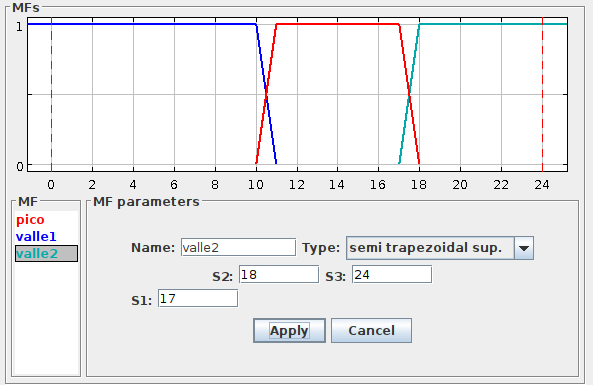
\includegraphics[scale=0.5]{./Images/hora_publicacion.png}
	\end{figure}
	\item \textbf{Relevancia de la temática en la actualidad (T)}: la relevancia de una temática en particular puede ser baja, media o alta y está representada por un índice del 0 al 1.
	\begin{figure}[H]
		\centering
		\includegraphics[scale=0.55]{./Images/relevancia_temática.png}
	\end{figure}
	\item \textbf{Cantidad de perfiles de prueba (C)}: hace referencia a la cantidad de perfiles a los que se le muestra el video en una primera instancia, y varía de 10 a 10000. La cantidad de perfiles de prueba es poca si es menor de 1500, es media si está entre 4000 y 6000, y es alta si es igual o mayor a 8500.
	\begin{figure}[H]
		\centering
		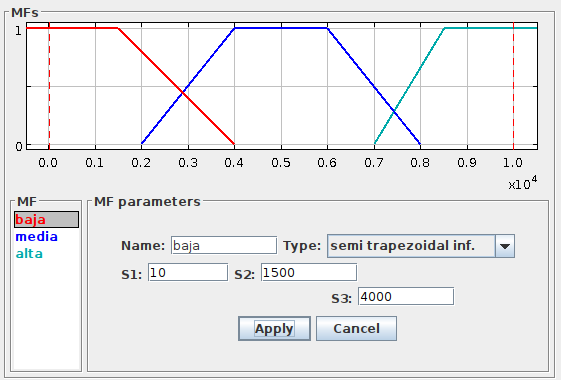
\includegraphics[scale=0.5]{./Images/perfiles_prueba_cant.png}
	\end{figure}
	\item \textbf{Duración del video (D)}: medido en cantidad de minutos, se puede decir que es corta, media o larga y va desde 0 a 10 minutos, siendo corta de 0 a 1 minuto, media de 1 a 3 minutos y larga si es mayor de 3 minutos.
	\begin{figure}[H]
		\centering
		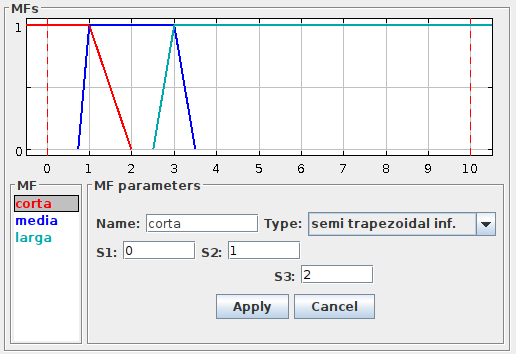
\includegraphics[scale=0.6]{./Images/duracion_video.png}
	\end{figure}
	\item \textbf{Tipo de interacción con el video (I)}: medida como el porcentaje de perfiles de prueba que tuvieron una o más interacciones positivas sobre el video. Se considera negativa si es menor al $5\%$, regular si es alrededor del $10\%$ y positiva si es más del $20\%$.
	\begin{figure}[H]
		\centering
		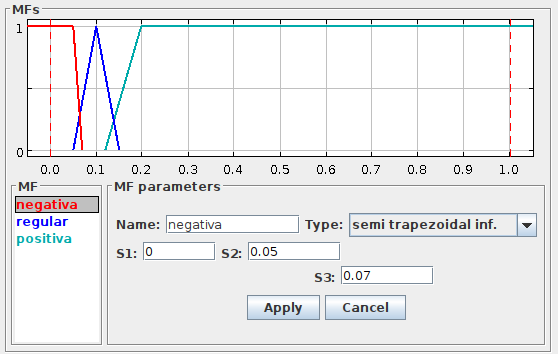
\includegraphics[scale=0.55]{./Images/tipo_interaccion.png}
	\end{figure}
	\item \textbf{Popularidad del video (P)}: para representar esta variable lingüística se utilizan 4 conjuntos borrosos definidos a partir de un índice del 0 al 1. Estos son: impopular (de 0 a 0.25), semi-popular (de 0.4 a 0.5), popular (de 0.7 a 0.8) y viral (mayor a 0.9).
	\begin{figure}[H]
		\centering
		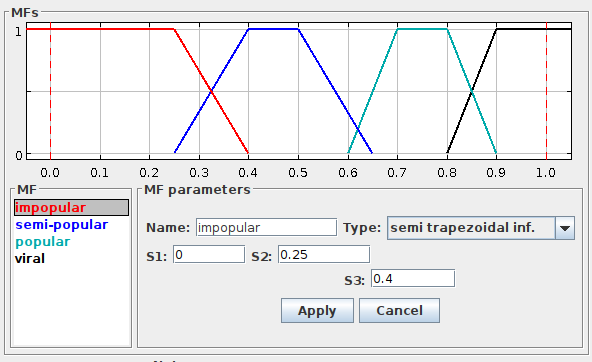
\includegraphics[scale=0.55]{./Images/popularidad.png}
	\end{figure}
\end{itemize}

\subsection{Reglas de inferencia}

Planteamos las reglas de inferencia utilizando la aritmética lógica adaptada al lenguaje natural, para presentarlas de forma compacta. 

\begin{itemize}
	\item Reglas relativas a la primera etapa
	\begin{itemize}
		\item [\textbf{R1}] H hora pico y T alta o media $\rightarrow$ C alta 
		\item [\textbf{R2}] H hora pico o valle y T baja $\rightarrow$ C poca 
		\item [\textbf{R3}] H hora valle y T alta o media $\rightarrow$ C media 
	\end{itemize}
	\item Reglas relativas a la segunda etapa
	\begin{itemize}
		\item [\textbf{S1}] C alta, D corta e I positiva $\rightarrow$ P viral
		\item [\textbf{S2}] C media, D corta o media e I positiva $\rightarrow$ P popular
		\item [\textbf{S3}] C alta, D media e I positiva $\rightarrow$ P popular
		\item [\textbf{S4}] C media, D larga e I positiva $\rightarrow$ P semi-popular
		\item [\textbf{S5}] C poca o media, D media e I regular $\rightarrow$ P semi-popular
		\item [\textbf{S6}] I negativa $\rightarrow$ P impopular
	\end{itemize}
\end{itemize}


En la herramienta \verb|fispro|, algunas de estas operaciones lógicas no se soportan y entonces se plantean, en su lugar, un conjunto de reglas por cada una de ellas. Así es como quedaron planteadas las reglas de inferencia en esta herramienta:


\begin{figure}[H]
		\centering
		\includegraphics*[scale=0.31]{./Images/rules1.png}
		\caption{Reglas de la primera etapa}
\end{figure}
	
\begin{figure}[H]
		\centering
		\includegraphics*[scale=0.4]{./Images/rules2.png}
		\caption{Reglas de la segunda etapa}
\end{figure}


\section{Pruebas y ajustes de parámetros}

\subsection{Pruebas}

Definimos 4 casos de prueba según consideramos relevantes para comprobar el correcto funcionamiento del modelo armado. Estos son:

\begin{itemize}
	\item Ejemplo 1: Se busca determinar la cantidad de perfiles de prueba para un video publicado a las 20:00 sobre la guerra entre Rusia y Ucrania (un topico considerado como muy relevante actualmente, en particular le asignamos una relevancia de 0.9).
 	\item Ejemplo 2: Se quiere determinar la cantidad de perfiles de prueba para un video publicado a las 17:18 sobre el último partido de la Selección Argentina de Fútbol (considerado como un tema relevante, en particular le asignamos una relevancia de 0.7).
	\item Ejemplo 3: Según el valor crisp obtenido en el ejemplo 1, determinar la popularidad de dicho video, siendo que dura 2.8 minutos (2 minutos 48 segundos) y en general tuvo una interaccion del $18\%$ por parte de los usuarios.
	\item Ejemplo 4: Según el valor crisp obtenido del ejemplo 2, determinar la popularidad de dicho video, que recibió una interaccion del $30\%$ y dura 0.9 minutos (54 segundos). También calcular su popularidad si por el contrario durase 2.5 minutos (2 minutos 30 segundos).
\end{itemize}

\subsection{Ajustes de parámetros}

Para los casos de prueba que requieren inferir la cantidad de perfiles de prueba a los que mostrarle el video (ejemplos 1 y 2), utilizamos de fuzzificador la T-norma producto algebraico y para los casos de prueba que requieren calcular la popularidad que alcanzaría dicho video (ejemplos 3 y 4), utilizamos la T-norma de Lukasiewicz, diferenca acotada. 
Ambas operaciones son altamente restrictivas y así fueron elegidas para acercarnos lo más posible al determinismo que hay detrás de la mayoría de los algoritmos de este estilo que son usados por las redes sociales. 
Para defuzzificar utilizamos, en todos los casos, el método mean max.

\section{Resultados}

\subsection*{Ejemplo 1}

Se busca determinar la cantidad de perfiles de prueba para un video publicado a las 20:00 sobre la guerra entre Rusia y Ucrania (un topico considerado como muy relevante actualmente, en particular le asignamos una relevancia de 0.9).

Inferencia del caso de estudio en la herramienta fispro:
\begin{figure}[H]
	\centering
	\includegraphics*[scale=0.35]{./Images/p1.png}
\end{figure}

La regla que se activó en este caso fue \textbf{R3}, como se esperaba. La cantidad de perfiles de prueba que se obtuvieron fue de 5500, valor que pertenece al conjunto borroso \verb|cantidad de perfiles de prueba media| con un grado de pertenencia de 1.

\subsection*{Ejemplo 2}

Se quiere determinar la cantidad de perfiles de prueba para un video publicado a las 17:18 sobre el último partido de la Selección Argentina de Fútbol (considerado como un tema relevante, en particular le asignamos una relevancia de 0.7).

Inferencia del caso de estudio en la herramienta fispro:
\begin{figure}[H]
	\centering
	\includegraphics*[scale=0.35]{./Images/p3.png}
\end{figure}

Las reglas que se activaron en este caso fueron \textbf{R1} y \textbf{R3}, pero la regla \textbf{R1} en mayor medida, como era de esperar. La cantidad de perfiles de prueba que se obtuvo fue de 9600, valor que pertenece al conjunto borroso \\ \verb|cantidad de perfiles de prueba alta| con un grado de pertenencia de 1.

\subsection*{Ejemplo 3}

Según el valor crisp obtenido en el ejemplo 1, determinar la popularidad de dicho video, siendo que dura 2.8 minutos (2 minutos 48 segundos) y en general tuvo una interaccion del $18\%$ por parte de los usuarios.

Inferencia del caso de estudio en la herramienta fispro:
\begin{figure}[H]
	\centering
	\includegraphics*[scale=0.32]{./Images/p2.png}
\end{figure}

Las reglas que se activaron en este caso fueron \textbf{S2} y \textbf{S4}, pero la regla \textbf{S2} en mayor medida, como era de esperar. La popularidad del video predecida fue de 0.75, valor que pertenece al conjunto borroso \verb|popularidad del video popular| con un grado de pertenencia de 1.

\subsection*{Ejemplo 4}

Según el valor crisp obtenido del ejemplo 2, determinar la popularidad de dicho video, que recibió una interaccion del $30\%$ y dura 0.9 minutos (54 segundos). También calcular su popularidad si por el contrario durase 2.5 minutos (2 minutos 30 segundos).

Inferencia del caso de estudio en la herramienta fispro:
\begin{figure}[H]
\begin{subfigure}[b]{0.3\textwidth}
	\centering
	\includegraphics*[scale=0.32]{./Images/p4-1.png}
	\caption{Situación 1}
\end{subfigure}

\begin{subfigure}[b]{0.3\textwidth}
	\centering
	\includegraphics*[scale=0.32]{./Images/p4-2.png}
	\caption{Situación 2}
\end{subfigure}
\end{figure}

En la primera situación, las reglas que se activaron fueron \textbf{S1} y \textbf{S3}, pero la regla \textbf{S1} en mayor medida, como se esperaba. La popularidad del video predecida fue de 1, valor que pertenece al conjunto borroso \verb|popularidad del video viral| con un grado de pertenencia de 1.

En la segunda situación, la regla que se activó fue solo \textbf{S3} y en este caso la popularidad del video predecida fue de 0.75, valor que pertenece al conjunto borroso \verb|popularidad del video popular| con un grado de pertenencia de 1.

De estos resultados en particular, se puede deducir claramente que la duración del video tiene una importante incidencia en la determinación de la popularidad de dicho video.


\section{Conclusiones}

La motivación para plantear este problema fue la de pensar y modelar los factores influyentes a la hora
de determinar el grado de viralidad de un video. Esto devino principalmente de la lectura de distintos estudios relacionados, destacándose el caso de \href{https://arxiv.org/abs/2012.07716}{\#TulsaFlop: A Case Study of Algorithmically-Influenced Collective Action on TikTok},
que analiza estadísticamente distintos vídeos de activismo social y su performance en TikTok.
Creemos que el modelo resulto propicio y nos permitió verificar nuestras intuiciones, mostrándonos como algunos pequeños cambios pueden afectar sustancialmente el desempeño de un vídeo
y otros pueden no hacerlo en igual medida.


\end{document}